% Created 2022-10-26 Wed 23:14
% Intended LaTeX compiler: pdflatex
\documentclass[a4paper,11pt]{article}
\usepackage[utf8]{inputenc}
\usepackage[T1]{fontenc}
\usepackage{graphicx}
\usepackage{grffile}
\usepackage{longtable}
\usepackage{wrapfig}
\usepackage{rotating}
\usepackage[normalem]{ulem}
\usepackage{amsmath}
\usepackage{textcomp}
\usepackage{amssymb}
\usepackage{capt-of}
\usepackage{hyperref}
\usepackage[margin=1in]{geometry}
\usepackage{titlesec}
\usepackage{caption}
\usepackage{subcaption}
\usepackage{lipsum}
\author{Varghese Reji}
\date{}
\title{Classical and Quantum Optics\\\medskip
\large Assignment-1 Answers}
\hypersetup{
 pdfauthor={Varghese Reji},
 pdftitle={Classical and Quantum Optics},
 pdfkeywords={},
 pdfsubject={},
 pdfcreator={Emacs 27.1 (Org mode 9.3)}, 
 pdflang={English}}
\begin{document}

\maketitle

\section*{Problem 1}
\label{sec:org528eb84}
\begin{description}
\item[{(a)}] We know that,
\end{description}
\begin{equation}
\label{eq:org98e5e05}
\mathcal{F}\{g(x,y)\} = \int_{-\infty}^\infty \int_{-\infty}^\infty dxdy g(x,y) e^{-2\pi i(f_Xx+f_Yy)}
\end{equation}

Then, we can write,
 $$\mathcal{F}\mathcal{F}\{g(x,y)\} = \int_{-\infty}^\infty \int_{-\infty}^\infty df_X df_Y ~e^{-2\pi i(f_Xx+f_Yy)} \int_{-\infty}^\infty \int_{-\infty}^\infty dx'dy' ~g(x',y') e^{-2\pi i(f_Xx'+f_Yy')}$$

By interchanging the order of integration,

 \begin{equation}
\label{eq:org1ba709a}
\begin{split}
\mathcal{F}\mathcal{F}\{g(x,y)\} = & \int_{-\infty}^\infty \int_{-\infty}^\infty dx'dy'~g(x',y') \int_{-\infty}^\infty \int_{-\infty}^\infty df_Xdf_Ye^{-2\pi i(f_X(x'+x)+f_Y(y'+y))} \\
\end{split}
\end{equation}

But we have the identity,

\begin{equation}
\label{eq:org57c866d}
\delta(x-x') = \frac{1}{2\pi} \int_{-infty}^\infty dp e^{ip(x-x')}
\end{equation}

Using this, we can write \ref{eq:org1ba709a} as
 \begin{equation}
\begin{split}
\mathcal{F}\mathcal{F}\{g(x,y)\} = & \int_{-\infty}^\infty \int_{-\infty}^\infty dx'dy'~g(x',y') \delta(x+x',y+y') \\
= & g(-x,-y)
\end{split}
\end{equation}

So, we can write, $$\mathcal{F}\mathcal{F}\{g(x,y)\} = g(-x,-y)$$

Similerly,

\begin{equation*}
\begin{split}
\mathcal{F}^{-1}\mathcal{F}^{-1}\{g(x,y)\} = & \int_{-\infty}^\infty \int_{-\infty}^\infty df_X df_Y ~e^{2\pi i(f_Xx+f_Yy)} \int_{-\infty}^\infty \int_{-\infty}^\infty dx'dy' ~g(x',y') e^{2\pi i(f_Xx'+f_Yy')}\\
= & \int_{-\infty}^\infty \int_{-\infty}^\infty dx'dy'~g(x',y') \int_{-\infty}^\infty \int_{-\infty}^\infty df_Xdf_Ye^{2\pi i(f_X(x'+x)+f_Y(y'+y))} \\
= & \int_{-\infty}^\infty \int_{-\infty}^\infty dx'dy'~g(x',y') \delta(x+x',y+y') \\
= & g(-x,-y)
\end{split}
\end{equation*}

Then,

$$\mathcal{F}\mathcal{F}\{g(x,y)\} = \mathcal{F}^{-1}\mathcal{F}^{-1}\{g(x,y)\} = g(-x,-y)$$

\begin{description}
\item[{(b)}] We can write the convolution of two functions as
\end{description}

\begin{equation}
\label{eq:org6bbb7f2}
g(t)\otimes h(t) = \int_{-\infty}^{\infty} d\tau~g(\tau) h(t-\tau)
\end{equation}

So, the given fucntion can be written as

$$\mathcal{F}\{g(x,y)\} \otimes \mathcal{F}\{h(x,y)\} = G(f_X,f_Y) \otimes H(f_X,f_Y) $$

Using equation \ref{eq:org6bbb7f2}, we can write this as,
\begin{equation}
\label{eq:org335736d}
G(f_X,f_Y) \otimes H(f_X,f_Y) = \int_{-\infty}^{\infty} \int_{-\infty}^{\infty} dF_X dF_Y G(F_X,F_Y) H(f_X-F_X,f_Y-F_Y)
\end{equation}

Let us take the inverse transform of this.

\begin{equation*}
\begin{split}
& \mathcal{F}^{-1}  \{G(f_X,f_Y)\otimes H(f_X,f_Y)\} \\ = & \mathcal{F}^{-1}\int_{-\infty}^{\infty} \int_{-\infty}^{\infty} dF_X dF_Y G(F_X,F_Y) H(f_X-F_X,f_Y-F_Y) \\
= & \int_{-\infty}^{\infty} \int_{-\infty}^{\infty} dF_X dF_Y G(F_X,F_Y) \mathcal{F}^{-1}\{H(f_X-F_X,f_Y-F_Y)\} \\
= & \int_{-\infty}^{\infty}\int_{-\infty}^{\infty} dF_X dF_Y G(F_X,F_Y) \exp\left(2\pi i\left[F_Xx+F_Yy\right]\right) \\  & ~~~~~~~~ \int_{-\infty}^{\infty} \int_{-\infty}^{\infty} df_X df_Y H(f_X-F_X,f_Y-F_Y)\exp\left(2\pi i\left[(f_X-F_X)x+(f_Y-F_Y)y\right] \right) \\
= & \int_{-\infty}^{\infty} \int_{-\infty}^{\infty} dF_X dF_Y G(F_X,F_Y) h(x,y) \\
= & g(x,y) h(x,y)
\end{split}
\end{equation*}

\(\therefore\)

$$\mathcal{F}\{g(x,y)f(x,y) = \mathcal{F}\{g(x,y)\}\otimes \mathcal{F}\{h(x,y)\}$$

\begin{description}
\item[{(c)}] $$\mathcal{F}\{\nabla^2g(x,y)\}=-4\pi^2(f_x^2+f_y^2)\mathcal{F}\{g(x,y)\}$$
\end{description}

We know that:

\begin{equation}
\label{eq:orgc15323c}
\int_V\left(\psi\vec{\nabla}^2\phi+\vec{\nabla}\psi\cdot\vec{\nabla}\phi\right)dV=\oint_S\psi\vec{\nabla}\phi\cdot d\vec{S}
\end{equation}

Let us take \(\psi = e^{-2\pi i\left(f_xx+f_yy\right)}\) and \(\phi = g(x,y)\).

But here, we can assume that value of \(g\) is really small at large \(x\) and \(y\). Gradiance of it also can be neglected. So the RHS of equ \ref{eq:orgc15323c} will be 0 when we take the closed integral along a large closed surface which includes the volume of integration in LHS.

Then, we can write,
\begin{equation}
\label{eq:org277282e}
\begin{split}
\int_V\psi\vec{\nabla}^2\phi dV= & -\int_V\vec{\nabla}\psi\cdot\vec{\nabla}\phi dV \\
= & \int_V\phi\vec{\nabla}^2\psi dV 
\end{split}
\end{equation}

Then, we can write,

\begin{equation*}
\label{eq:orgf323a18}
\begin{split}
\mathcal{F}(\nabla^2g(x,y)) = & \int_{-\infty}^\infty dxdy~ e^{-2\pi i(f_Xx+f_Xx)}\nabla^2g(x,y) \\ = & \int_{-\infty}^\infty dxdy~ g(x,y)\nabla^2e^{-2\pi i(f_Xx+f_Xx)} \\ 
= & -4\pi^2(f_X^2+f_Y^2) \int_{-\infty}^\infty dxdy~ g(x,y)\nabla^2e^{-2\pi i(f_Xx+f_Xx)} \\
= & -4\pi^2(f_X^2+f_Y^2)\mathcal{F}\{g(x,y)\}
\end{split}
\end{equation*}

\newpage
\section*{Problem 2}
\label{sec:org396d2ab}
\begin{description}
\item[{(a)}] Given \(g_R(r)=\delta(r-r_0)\).
\end{description}

$$g(u,v)=\int_{-\infty}^{\infty}\int_{-\infty}^{\infty} f(r) e^{-2\pi i\left(ux+vy\right)} dxdy$$

Let us take,

\begin{equation*}
\begin{split}
x+iy = & re^{i\theta}\\
u+iv = & \rho e^{i\phi}
\end{split}
\end{equation*}

Then,

\begin{equation*}
\begin{split}
x = & r\cos\theta\\
y = & r\sin\theta\\
r = & \sqrt{x^2+y^2}\\
u = & \rho\cos\phi\\
v = & \rho\sin\phi \\
\rho = & \sqrt{u^2+v^2}
\end{split}
\end{equation*}

Then, we can write,

\begin{equation*}
\begin{split}
g(\rho) = & \int_0^\infty\int_0^{2\pi} f(r)e^{-2\pi ir\rho\left(\cos\phi\cos\theta+\sin\phi\sin\theta\right)}rdrd\theta \\
= & \int_0^\infty\int_0^{2\pi} f(r)e^{-2\pi ir\rho\cos\left(\theta-\phi\right)} rdrd\theta \\
= & \int_0^\infty\int_{-\phi}^{2\pi-\phi} f(r)e^{-2\pi ir\rho\cos\theta}rdrd\theta \\
= & \int_0^\infty\int_{0}^{2\pi} f(r)e^{-2\pi ir\rho\cos\theta}rdrd\theta \\
= & \int_0^\infty f(r) \left[\int_0^{2\pi}e^{-2\pi ir\rho\cos\theta}d\theta\right]rdr \\
= & 2\pi\int_0^\infty f(r)J_0\left(2\pi \rho r\right) rdr
\end{split}
\end{equation*}

So,

\begin{equation}
\label{eq:orgc6445f3}
g(\rho) = 2\pi\int_0^\infty f(r)J_0\left(2\pi \rho r\right) rdr
\end{equation}


Here, \(f(r)=g_R(r)=\delta(r-r_0)\).

Then, 

\begin{equation*}
\begin{split}
\mathcal{B}\{g_R(r)\} = & g(\rho) \\
= & 2\pi\int_0^\infty f(r)J_0\left(2\pi \rho r\right) rdr \\
= & 2\pi\int_0^\infty \delta(r-r_0)J_0\left(2\pi \rho r\right) rdr \\
= & 2\pi r_0J_0\left(2\pi \rho r_0\right)
\end{split}
\end{equation*}

\(\therefore\)

$$\mathcal{B}\{g_R(r)\} = 2\pi r_0J_0\left(2\pi \rho r_0\right) $$

\begin{description}
\item[{(b)}] \(g_R(r) = 1 for a\leq r \leq 1\) and zero elsewhere.
\end{description}

We have the identity,

\begin{equation}
\label{eq:orgae3051c}
\int_0^x x'J_0(x') dx' = xJ_1(x)
\end{equation}

So,

\begin{equation*}
\begin{split}
\mathcal{B}\{g_R(r)\} = & 2\pi \int_a^1 J_0\left(2\pi \rho r\right) rdr \\
= & 2\pi\left[ \int_0^1 J_0\left(2\pi \rho r\right) rdr -  \int_0^a J_0\left(2\pi \rho r\right) rdr\right]\\
= & \frac{1}{2\pi\rho^2}\left[ \int_0^1 J_0\left(2\pi \rho r\right) (2\pi\rho r)(2\pi\rho dr) -  \int_0^a J_0\left(2\pi \rho r\right) (2\pi\rho r)(2\pi\rho dr)\right]\\
\end{split}
\end{equation*}

Let, \(x = 2\pi\rho r\). Then, when \$r=a, \(x=2\pi\rho a\). \(\Rightarrow\) \(a=\frac{x}{2\pi\rho}\). Apply same for \(r=1\).

Then,

\begin{equation*}
\begin{split}
\mathcal{B}\{g_R(r)\} = & \frac{1}{4\pi^2\rho^2}\left[ \int_0^{1} J_0\left(2\pi \rho r\right) (2\pi\rho r)(2\pi\rho dr) -  \int_0^a J_0\left(2\pi \rho r\right) (2\pi\rho r)(2\pi\rho dr)\right]\\
= & \frac{1}{2\pi\rho^2} \left[\int_0^{2\pi\rho} J_0\left(x\right) xdx - \int_0^{2\pi\rho a} J_0\left(x\right) xdx\right] \\
= &  \frac{1}{2\pi\rho^2}\left[2\pi\rho J_1(2\pi\rho)-2\pi\rho a J_1(2\pi\rho a)\right] \\
= &  \frac{1}{\rho}\left[J_1(2\pi\rho)-a J_1(2\pi\rho a)\right]
\end{split}
\end{equation*}


\(\therefore\)

$$\mathcal{B}\{g_R(r)\}=\frac{J_1(2\pi\rho)-a J_1(2\pi\rho a)}{\rho}$$

\begin{description}
\item[{(c)}] Given, \(\mathcal{B}\{g_R(r)\} = G(\rho)\).
\end{description}

From equ \ref{eq:orgc6445f3}, $$g(\rho) = 2\pi\int_0^\infty g_R(r)J_0\left(2\pi \rho r\right) rdr $$

Here, \(g_R(r)\rightarrow g_R(ar)\)
\(\Rightarrow\)

\begin{equation*}
\begin{split}
\mathcal{B}\{g_R(ar)\} = &  2\pi\int_0^\infty g_R(ar)J_0\left(2\pi \rho r\right) rdr \\ 
= &  2\pi\int_0^\infty g_R(ar)J_0\left(2\pi a \left(\frac{\rho}{a}\right) r\right) \left(\frac{ar}{a}\right)\frac{adr}{a} \qquad\qquad (ra\rightarrow x) \\ 
= &  \frac{1}{a^2}2\pi\int_0^\infty g_R(a)J_0\left(2\pi  \left(\frac{\rho}{a} x\right)\right) xdx \\
= & \frac{1}{a^2}G\left(\frac{\rho}{a}\right)
\end{split}
\end{equation*}

Hence, 

$$\mathcal{B}\{g_R(ar)\} = \frac{1}{a^2}G\left(\frac{\rho}{a}\right)$$

\begin{description}
\item[{(d)}] Fourier-Bessel transform is basically Fourier transform of 2-D functions with circular symmetry. So, we can do the FT of given function in cartesian coordinate also.
\end{description}

Given function is \(g_R(r)=\exp\left(-\pi r^2\right)=\exp\left(-\pi(x^2+y^2\right)\).

This is variable separable. So, we can take the Fourier transform of individuals. Then, we will get,
\begin{equation*}
\begin{split}
\mathcal{F}\{\exp\left(-\pi(x^2+y^2)\right) = \mathcal{F}\{\exp(-\pi x^2)\}\mathcal{F}\{\exp(-\pi y^2)\} \\
= & \exp(-\pi f_X^2)\exp(-\pi f_Y^2) \\
= & \exp\left(-\pi(f_X^2+f_Y^2)\right)
\end{split}
\end{equation*}

But, \(f_X^2+f_Y^2=\rho^2\)

\(\therefore\),

$$\mathcal{B}\{\exp(-\pi r^2)\} = \exp(-\pi \rho^2) $$

\newpage
\section*{Problem 3}
\label{sec:org2b24e3a}
\begin{equation}
W(f,x) = \int_{-\infty}^{\infty} g(x+\frac{\xi}{2})g^*(x-\frac{\xi}{2})\exp(-j2\pi f\xi) d\xi
\end{equation}
\begin{description}
\item[{(a)}] \(g(x) = \exp(j\pi \beta x^2)\)
\end{description}

\begin{equation*}
\begin{split}
W(f,x) = & \int_{-\infty}^{\infty} \exp\left[j\pi\beta \left(x+\frac{\xi}{2}\right)^2\right]\exp\left[-j\pi\beta \left(x-\frac{\xi}{2}\right)^2\right]\exp(-j2\pi f\xi) d\xi \\
= & \int_{-\infty}^{\infty} \exp\left[j\pi\beta \left[\left(x+\frac{\xi}{2}\right)^2 - \left(x-\frac{\xi}{2}\right)^2\right]\right]\exp(-j2\pi f\xi) d\xi \\
\end{split}
\end{equation*}

\begin{equation*}
\begin{split}
\left(x+\frac{\xi}{2}\right)^2 - \left(x-\frac{\xi}{2}\right)^2 = & x^2+x\xi + \frac{\xi^2}{4} - x^2+x\xi - \frac{\xi^2}{4} \\
= & 2x\xi
\end{split}
\end{equation*}

\(\Rightarrow\)

\begin{equation*}
\begin{split}
W(f,x) = & \int_{-\infty}^{\infty} \exp\left[j\pi \beta \left[\left(x+\frac{\xi}{2}\right)^2 - \left(x-\frac{\xi}{2}\right)^2\right]\right]\exp(-j2\pi f\xi) d\xi \\
 = & \int_{-\infty}^{\infty} \exp\left[j2\pi \beta x\xi\right]\exp(-j2\pi f\xi) d\xi \\
 = & \int_{-\infty}^{\infty} \exp\left[j2\pi(\beta x-f)\xi\right] d\xi \\
 = & \delta(f-\beta x)
\end{split}
\end{equation*}

\(\therefore\)

$$W(f,x) = \delta(f-\beta x) $$

\begin{description}
\item[{(b)}] \(g(x) = \exp(j\pi \beta x^2)\text{rect}\left(\frac{x}{2L}\right)\)
\end{description}

\begin{equation*}
\begin{split}
W(f,x) = & \int_{-\infty}^{\infty} \exp\left[j\pi\beta \left(x+\frac{\xi}{2}\right)^2\right]\exp\left[-j\pi\beta \left(x-\frac{\xi}{2}\right)^2\right]\text{rect}\left(\frac{x+\frac{\xi}{2}}{2L}\right)\text{rect}\left(\frac{x-\frac{\xi}{2}}{2L}\right)\exp(-j2\pi f\xi) d\xi \\
 = & \int_{-\infty}^{\infty} \exp\left[j2\pi \beta x\xi\right]\text{rect}\left(\frac{x}{2L}+\frac{\xi}{4L}\right)\text{rect}\left(\frac{x}{2L}-\frac{\xi}{4L}\right)\exp(-j2\pi f\xi) d\xi \\
\end{split}
\end{equation*}

By the definition of rectangular function,
\begin{equation}
\label{eq:orgce6ae2d}
\Pi(x) = \begin{cases}
0 ~ \text{if}~& |x|>\frac{1}{2} \\
\frac{1}{2} ~ \text{if}~& |x|=\frac{1}{2} \\
1 ~ \text{if}~& |x|<\frac{1}{2} \\
\end{cases}
\end{equation}

By analysing it, we will get

\begin{equation}
\text{rect}\left(\frac{x}{2L}+\frac{\xi}{4L}\right)\text{rect}\left(\frac{x}{2L}-\frac{\xi}{4L}\right) = \text{rect}\left(\frac{\xi}{4(L-|x|)}\right)
\end{equation}


Then, we will get,

\begin{equation*}
\begin{split}
W(f,x) = & \int_{-\infty}^{\infty} \exp\left[j2\pi \beta x\xi\right]\text{rect}\left(\frac{x}{2L}+\frac{\xi}{4L}\right)\text{rect}\left(\frac{x}{2L}-\frac{\xi}{4L}\right)\exp(-j2\pi f\xi) d\xi \\
= & \int_{-\infty}^{\infty} \exp\left[j2\pi (\beta x-f)\xi\right]\text{rect}\left(\frac{\xi}{4(L-|x|)}\right)d\xi \\
= & [4(L-|x|)]\text{sinc}[4(L-|x|)(\beta x-f)]
\end{split}
\end{equation*}

\begin{description}
\item[{(c)}] The plots are given in figures \ref{fig:orga2461dc} and \ref{fig:orgf3c3f84}.
\end{description}

\begin{figure}[!htb]
\centering
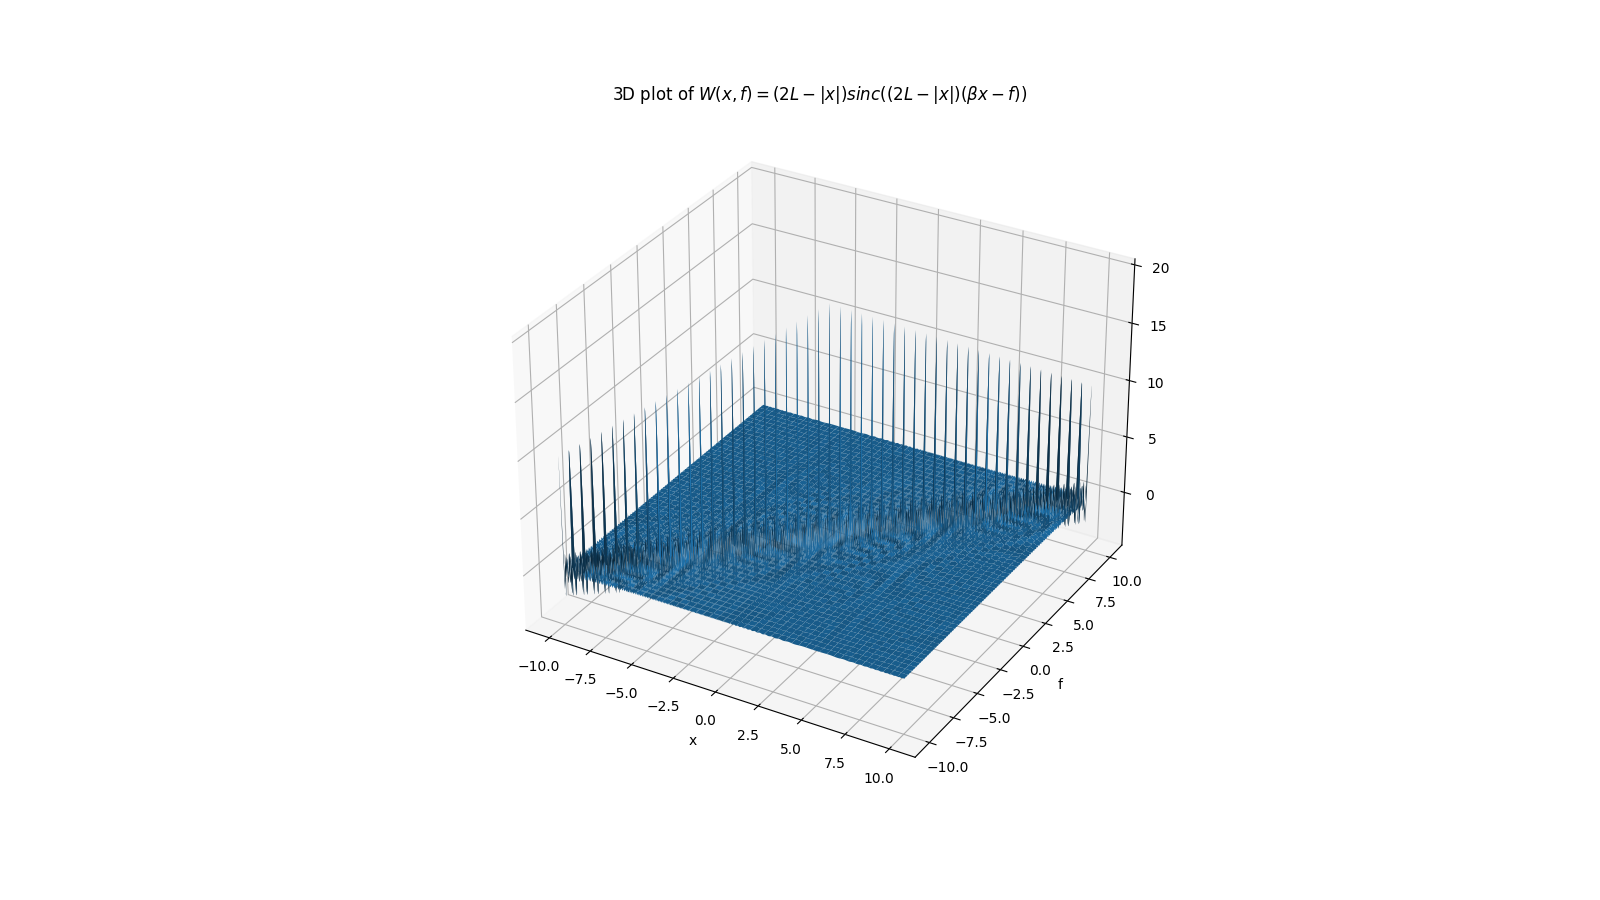
\includegraphics[width=17cm]{3D_plot.png}
\caption{\label{fig:orga2461dc}3D plot of \(W(f,x)= [4(L-|x|)]\text{sinc}[4(L-|x|)(\beta x-f)]\)}
\end{figure}

\begin{figure}[!htb]
\centering
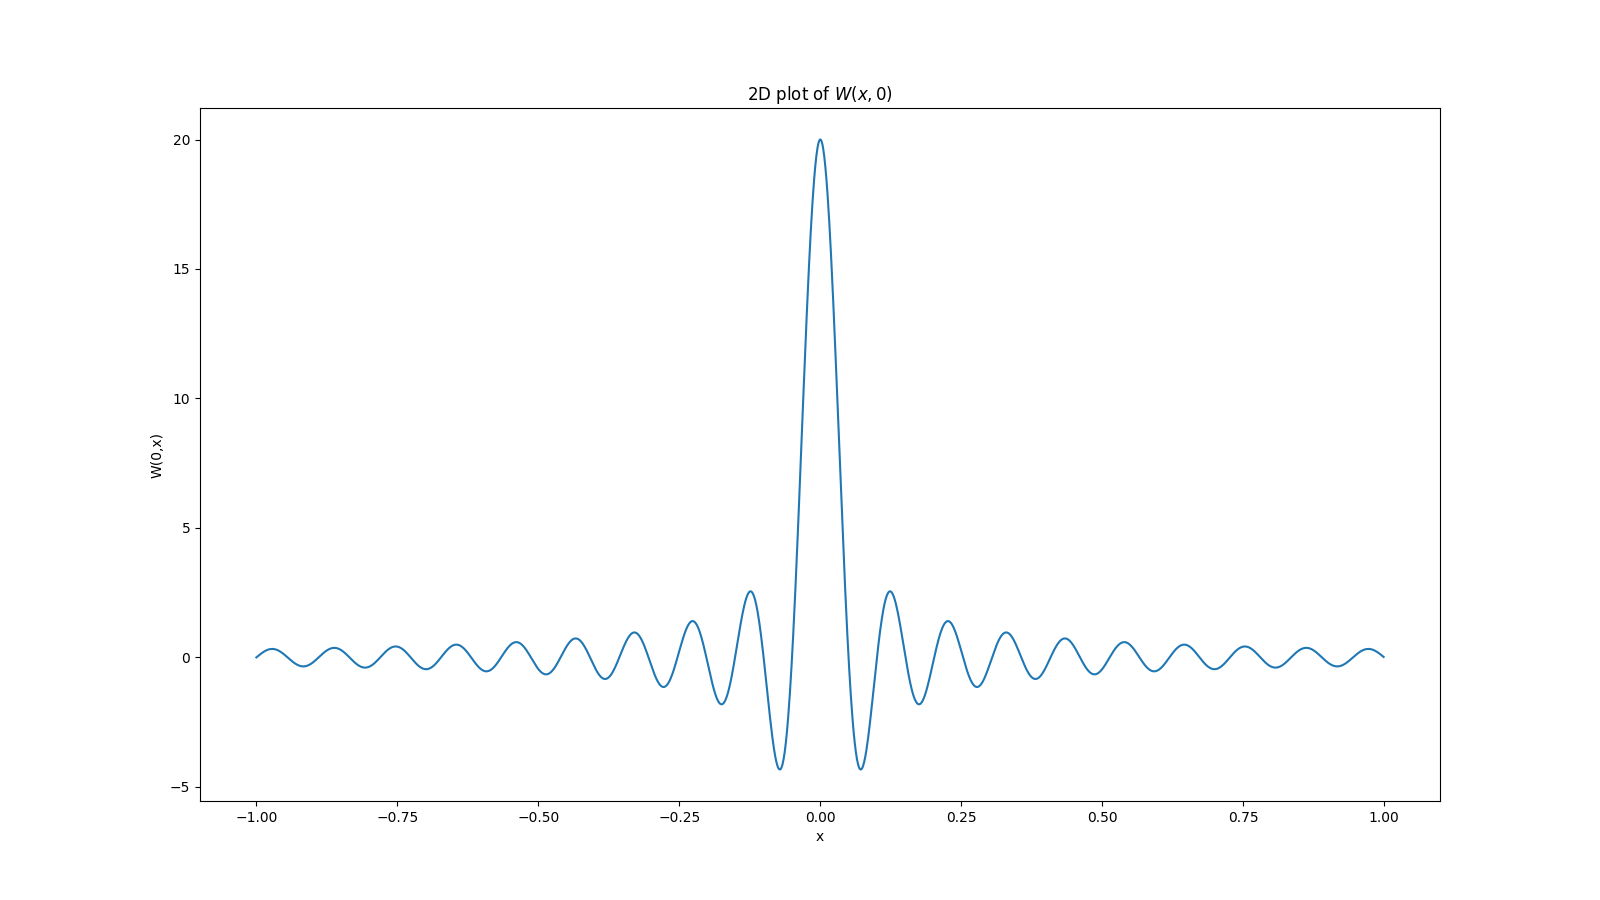
\includegraphics[width=17cm]{2D_plot.png}
\caption{\label{fig:orgf3c3f84}2D plot of \(W(0,x)= [4(L-|x|)]\text{sinc}[4(L-|x|)(\beta x)]\)}
\end{figure}
\newpage
\section*{Problem 4}
\label{sec:orgf03d483}
The grating is modeled as a transmitting structure with amplitude transmittance:
$$t_{A}(\xi,\eta) = \frac{1}{2}\left[1+m\cos\left(2\pi\frac{\xi}{L}\right)\right]$$

For more simplicity, we can assume that the grating structure is bounded by a square aperture of width \(2w\). \(m\) representa the peak-to-peak change of amplitude transmittance across the screen and \(f_0=\frac{1}{L}\) is the spatial frequency of the grating. Using these, we can modify \(t_A\).

\begin{equation}
\label{eq:orgf9fd229}
t_{A}(\xi,\eta) = \frac{1}{2}\left[1+m\cos\left(2\pi f_0\xi\right)\right]\text{rect}\left(\frac{\xi}{2w}\right)\text{rect}\left(\frac{\eta}{2w}\right)
\end{equation}

Let us say that the screen s normally illuminated by a unit-amplitude plane wave. The field distribution across the aperture is equal simply to \(t_A\). To find the Fraunhofer diffraction pattern, we first take the transform of \(t_A\).

$$\mathcal{F}\left[\frac{1}{2}\left[1+m\cos\left(2\pi f_0\xi\right)\right]\right] = \frac{1}{2}\delta(f_X,f_Y) +\frac{m}{4}\delta(f_X+f_0,f_Y) + \frac{m}{4}\delta(f_X-f_0,f_Y) $$
$$\mathcal{F}\left[\text{rect}\left(\frac{\xi}{2w}\right)\text{rect}\left(\frac{\eta}{2w}\right)\right] = A \text{sinc}(2wf_X)\text{sinc}(2wf_Y)$$

\(A\) is the area of the aperture bounding the grating. Using the convolution theorem, we can write that, The FT of \(U(\xi,\eta)\) is the product of equations that we got above.

\begin{equation}
\label{eq:org41a07a5}
\begin{split}
\mathcal{F}\{U(\xi,\eta)\} = & A \text{sinc}(2wf_X)\text{sinc}(2wf_Y) \left[ \frac{1}{2}\delta(f_X,f_Y) +\frac{m}{4}\delta(f_X+f_0,f_Y) + \frac{m}{4}\delta(f_X-f_0,f_Y)\right] \\
= & \frac{A}{2}\text{sinc}(2wf_Y)\left[\text{sinc}(2wf_X) +\frac{m}{2}\text{sinc}(2w(f_X+f_0)) + \frac{m}{2}\text{sinc}(2w(f_X-f_0))\right]
\end{split}
\end{equation}

Now, using the formula of diffraction pattern,

\begin{equation}
\label{eq:org6f83e14}
U(x,y) = \frac{e^{jkz}e^{j\frac{k}{2z}(x^2+y^2)}}{j\lambda z} \mathcal{F}\{U(\xi,\eta)\}
\end{equation}

the amplitude distribution of our diffraction will be,

\begin{equation}
\label{eq:orgdc7a724}
U(x,y) = \frac{Ae^{jkz}e^{j\frac{k}{2z}(x^2+y^2)}}{2j\lambda z}\text{sinc}(2w\frac{y}{\lambda z})\left[\text{sinc}(2w\frac{x}{\lambda z}) +\frac{m}{2}\text{sinc}(\frac{2w}{\lambda z}(x+f_0\lambda z)) + \frac{m}{2}\text{sinc}(\frac{2w}{\lambda z}(x-f_0\lambda z))\right]
\end{equation}

The intensity distribution will be the square of \ref{eq:orgdc7a724}.

\begin{equation}
\label{eq:orgd9f1865}
I(x,y) = \frac{A^2}{4\lambda^2 z^2}\text{sinc}^2(2w\frac{y}{\lambda z})\left[\text{sinc}(2w\frac{x}{\lambda z}) +\frac{m}{2}\text{sinc}(\frac{2w}{\lambda z}(x+f_0\lambda z)) + \frac{m}{2}\text{sinc}(\frac{2w}{\lambda z}(x-f_0\lambda z))\right]^2
\end{equation}

But if there are many grating periods within the aperture, then \(f_0>>\frac{1}{w}\). So, the cross term of sinc functions will be negligible. Therefore,

\begin{equation}
\label{eq:org2542a7b}
I(x,y) = \frac{A^2}{4\lambda^2 z^2}\text{sinc}^2(2w\frac{y}{\lambda z})\left[\text{sinc}^2(2w\frac{x}{\lambda z}) +\frac{m}{2}\text{sinc}^2(\frac{2w}{\lambda z}(x+f_0\lambda z)) + \frac{m}{2}\text{sinc}^2(\frac{2w}{\lambda z}(x-f_0\lambda z))\right]
\end{equation}

The width of each order will be \(\frac{\lambda z}{w}\). For, \(x=0\), it will be the central maximum. The one coming after that will be first order. 

\newpage
\section*{Problem 5}
\label{sec:orgee7c970}
We have the equation:
\begin{equation}
\label{eq:orge178954}
u_-(P,t) = \int_{-\infty}^{0} U(P,\nu)\exp(j 2\pi \nu t)d \nu
\end{equation}

U(P,\(\nu\)) is the Fourier spectrum of \(u(P,t)\).

\begin{figure}[htbp]
\centering
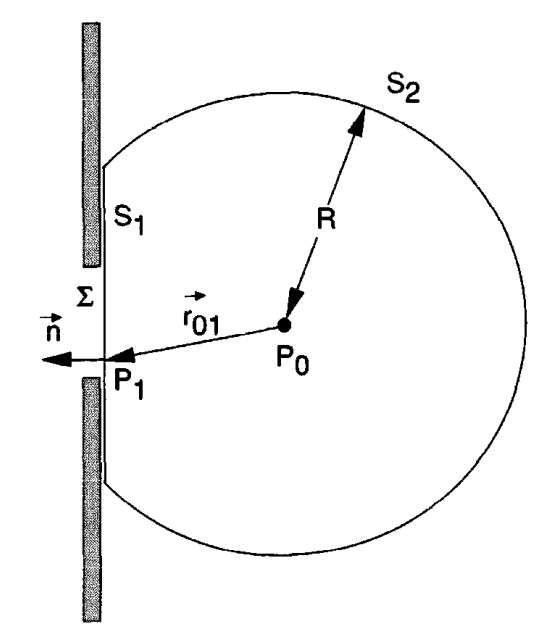
\includegraphics[width=4cm]{Pr_5_figure.png}
\caption{\label{fig:org6938c93}The surface}
\end{figure}

The figure is as showin in \ref{fig:org6938c93}.


We have the equation:

\begin{equation}
\label{eq:orgc1df80e}
\begin{split}
u_-(P_0,t) = \iint_{\Sigma} \frac{\cos(\vec{n},\vec{r}_{01})}{2\pi vr_{01}} \int_{-\infty}^{\infty} -j2\pi \nu' U(P_1,-\nu')\exp\left[-j2\pi\nu'\left(t-\frac{r_{01}}{v}\right)\right]d\nu' ds
\end{split}
\end{equation}

Here, the central frequency is \(\bar{\nu}\), and the bandwidth \(\Delta{\nu}\). So, the integral in the frequency is non-vanishing only in the range \(\left(\bar{\nu}-\frac{\Delta\nu}{2},\bar{\nu}+\frac{\Delta\nu}{2}\right)\). Given that \(\Delta\nu << \bar{\nu}\). So, the first \(\nu'\) will varie a small amount, since it is just linear in nature. We can replace that with \(\bar{\nu}\). Also \(\frac{1}{\Delta \nu} >> \frac{n r_{01}}{v}\). Then we can replace \(\nu'\) in the exponential with the term \(\frac{\nu'r_{01}}{v}\), by \(\bar{nu}\). We don't know the \(\nu'\) in other terms varie or that will make a huge difference in the result. Then, \ref{eq:orgc1df80e} will be,


\begin{equation*}
\begin{split}
u_-(P_0,t) = & \iint_{\Sigma} \frac{\cos(\vec{n},\vec{r}_{01})}{2\pi vr_{01}} \int_{-\infty}^{\infty} -j2\pi \bar{\nu} U(P_1,-\nu')\exp\left[-j2\pi\nu't\right]\exp\left[j2\pi\bar{\nu}\left(\frac{r_{01}}{v}\right)\right]d\nu' ds\\
= &-j2\pi \bar{\nu} \iint_{\Sigma}\exp\left[j2\pi\bar{\nu}\left(\frac{r_{01}}{v}\right)\right] \frac{\cos(\vec{n},\vec{r}_{01})}{2\pi vr_{01}} \int_{-\infty}^{\infty}  U(P_1,-\nu')\exp\left[-j2\pi\nu't\right]d\nu' ds\\
= &\frac{1}{\bar{j\lambda}} \iint_{\Sigma}\exp\left[j2\pi\bar{\nu}\left(\frac{r_{01}}{v}\right)\right] \frac{\cos(\vec{n},\vec{r}_{01})}{r_{01}} \int_{-\infty}^{\infty}  U(P_1,-\nu')\exp\left[-j2\pi\nu't\right]d\nu' ds\\
= &\frac{1}{\bar{j\lambda}} \iint_{\Sigma}\exp\left[j2\pi\bar{\nu}\left(\frac{r_{01}}{v}\right)\right] \frac{\cos(\vec{n},\vec{r}_{01})}{r_{01}} u_-(P_1,t) ds~~~~~~~~~~\text{(Using equation 3-55 in Goodman)}.
\end{split}
\end{equation*}

But, outside sigma, we can say that \(u_-(P_1,t)\) will be zero. Then, we can make the integral upto infinity. So, we will get the equation,

\begin{equation}
v_-(P_0,t)= \frac{1}{\bar{j\lambda}} \iint_{-\infty}^\infty \exp\left(j\bar{k} r_{01}\right) \frac{\cos(\vec{n},\vec{r}_{01})}{r_{01}} u_-(P_1,t) ds
\end{equation}

\newpage
\section*{Problem 6}
\label{sec:org7caf297}


The periodic triangular wave is given by

\begin{equation*}
y = |x| ~~~(-\pi < x \leq \pi )
\end{equation*}

A single wave can be written in the form,

\begin{equation}
\label{eq:org808bd77}
y = \begin{cases}
&x~ \text{if}~ 0\leq x<\pi \\
&-x~ \text{if}~ -\pi\leq x<0 \\
\end{cases}
\end{equation}

The period of wave is \(2\pi\).

We can write a periodic wave in the form,

\begin{equation}
\label{eq:org093d9f7}
g(t) = \sum_{n=-\infty}^{\infty} C_n e^{i 2\pi f_0 t} 
\end{equation}

Where \(C_n\) is the Fourier coefficients and defined by the formula:

\begin{equation}
\label{eq:org76b2d66}
C_n=\frac{1}{T}\int_{-\frac{T}{2}}^{\frac{T}{2}} g(t) e^{-i 2\pi n f_0t} dt
\end{equation}

\(f_0=\frac{1}{T}\)

Here, \(T=2\pi\). \(\therefore\)

\begin{equation*}
\begin{split}
C_n = & \frac{1}{2\pi} \left[\int_{-\pi}^0 (-x) e^{-i n x} dx + \int_{0}^{\pi} e^{-i nx} dx\right]\\
= & \frac{-1+e^{-i \pi  n} (1+i \pi  n)}{n^2}+\frac{-1+e^{i \pi  n} (1-i \pi  n)}{n^2} \\
= & \frac{-1+e^{-i \pi  n} (1+i \pi  n)-1+e^{i \pi  n} (1-i \pi  n)}{n^2}\\
= & \frac{-2+e^{-i \pi n}+i \pi n e^{-i \pi  n}+e^{i \pi n}-i \pi n e^{i \pi n}}{n^2} \\
= & \frac{-2+2\cos(n\pi)-2 \pi n \sin(n\pi)}{n^2} \\
= & 2\frac{ (-1)^n-1}{n^2}
\end{split}
\end{equation*}

Then, the Fourier transform of g(x) is,

\begin{equation*}
\begin{split}
G(f) = & \mathcal{F}\{g(x)\} \\
= & \sum_{n=-\infty}^{\infty}  2\frac{ (-1)^n-1}{n^2}\int_{-\infty}^{\infty} e^{i 2\pi (f-nf_0) x} dx   \\
= & \sum_{n=-\infty}^{\infty}  2\frac{ (-1)^n-1}{n^2} \delta(f-nf_0)   \\
\end{split}
\end{equation*}

So, the fourier transform of the given function can be written as:

$$G(f) = \sum_{n=-\infty}^{\infty}  2\frac{ (-1)^n-1}{n^2} \delta\left(f-\frac{n}{2\pi}\right)  $$

The signal and it's fourier transform is shown in figure \ref{fig:org049b13c}.

\begin{figure}[htbp]
\centering
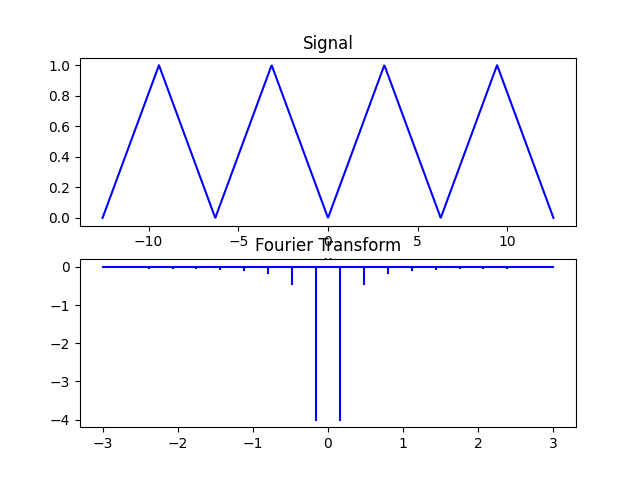
\includegraphics[width=.9\linewidth]{Pr6_signal_FT.png}
\caption{\label{fig:org049b13c}The signal and it's FT}
\end{figure}

\newpage
\section*{Problem 7}
\label{sec:org270d154}

Given function is a periodic array of \$\(\delta\)\$-function which every fifth member is missing. The function as showin in figure  \ref{fig:org3b5b9f1}

This can be considered as a wave train of group of 4 dirac delta functions. So, one complete wave can be written as:

\begin{equation}
\label{eq:orga10d5ff}
\Delta(x) = \delta(x+3)+\delta(x+1)+\delta(x-1)+\delta(x-3)
\end{equation}

The given function is a convolution of \(g(x)\) with the function

\begin{equation}
\label{eq:org6854040}
h(x) = \sum_{n=-\infty}^{\infty} \delta(x-5n)
\end{equation}

Now, let us write the given equation in the form of equation \ref{eq:org093d9f7}. Here, \(T=10\).

Then,

\begin{equation*}
\begin{split}
C_n = & \frac{1}{10}\int_{-5}^{5} dx e^{-\frac{2\pi n x}{10}} \left[ \delta(x+3)+\delta(x+1)+\delta(x-1)+\delta(x-3)\right] \\
= & \frac{1}{10} \left[e^{\frac{i6\pi n }{10}}+e^{\frac{-i6\pi n }{10}}+e^{\frac{i2\pi n }{10}}+e^{\frac{-i2\pi n }{10}}\right] \\
= & \frac{1}{5}\left[\cos\left(\frac{2\pi n}{5}\right)+\cos\left(\frac{\pi n}{5}\right)\right] \\
= & \frac{2}{5} \cos\left(\frac{3\pi n}{10}\right)\cos\left(\frac{\pi n}{10}\right)
\end{split}
\end{equation*}

\(\therefore\)

\begin{equation*}
\begin{split}
G(f) = & \mathcal{F}\{g(x)\} \\
= & \sum_{n=-\infty}^{\infty}  \frac{2}{5} \cos\left(\frac{3\pi n}{10}\right)\cos\left(\frac{\pi n}{10}\right)\int_{-\infty}^{\infty} e^{i 2\pi (f-nf_0) x} dx   \\
= & \sum_{n=-\infty}^{\infty}  \frac{2}{5} \cos\left(\frac{3\pi n}{10}\right)\cos\left(\frac{\pi n}{10}\right) \delta\left(f-\frac{n}{10}\right)
\end{split}
\end{equation*}

So, the Fourier transform is:

$$G(f) = \sum_{n=-\infty}^{\infty}  \frac{2}{5} \cos\left(\frac{3\pi n}{10}\right)\cos\left(\frac{\pi n}{10}\right) \delta\left(f-\frac{n}{10}\right)$$

The plot of signal and it's transform is shown in figure \ref{fig:org3b5b9f1}.

\begin{figure}[htbp]
\centering
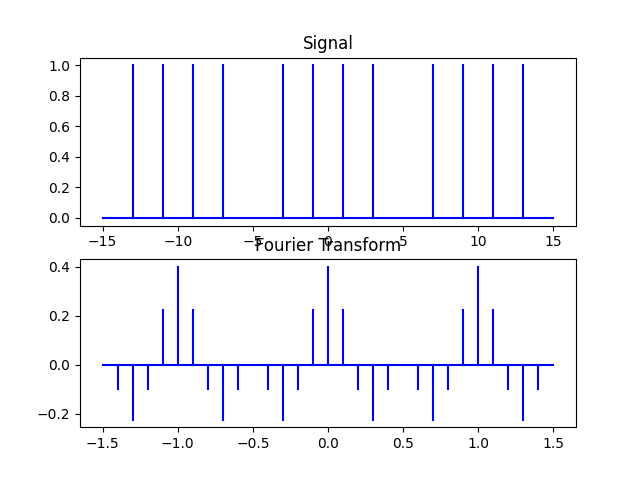
\includegraphics[width=.9\linewidth]{Pr7_Signal_Transform.png}
\caption{\label{fig:org3b5b9f1}Signal and Frequency Spectrum}
\end{figure}
\newpage
\section*{Problem 8}
\label{sec:org7246eb5}

\begin{figure}[htbp]
\centering
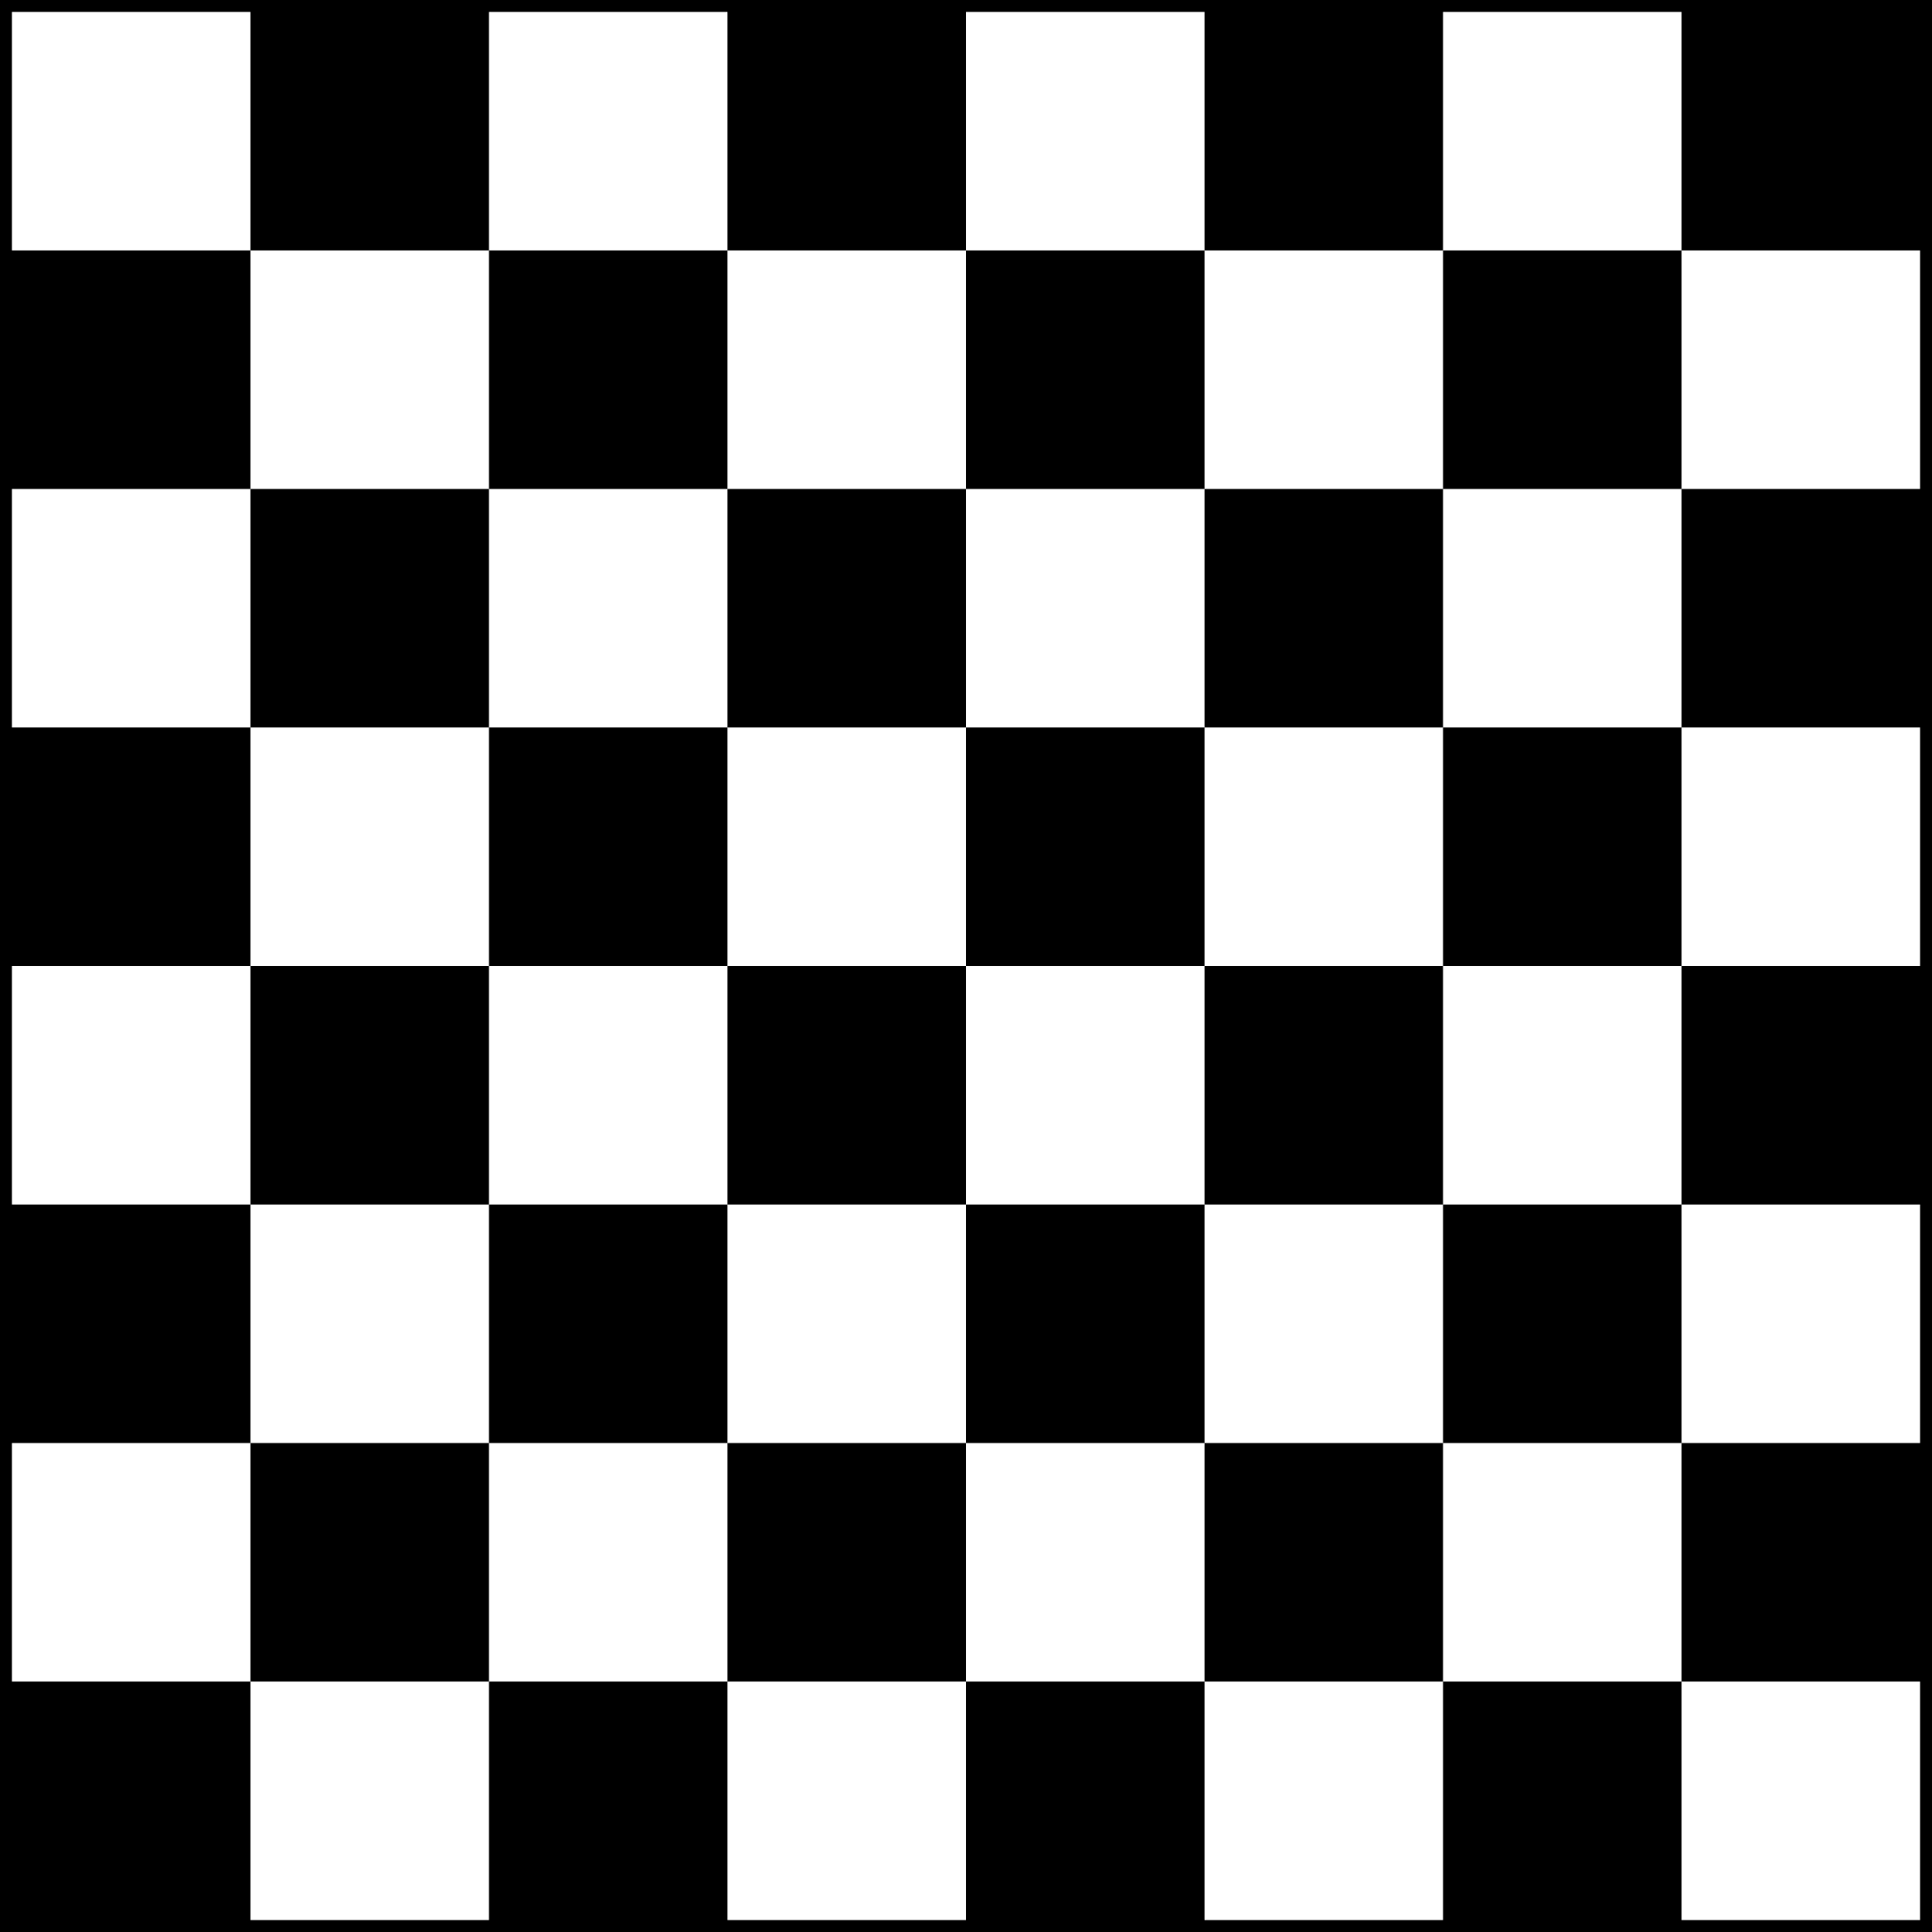
\includegraphics[width=6cm]{Chess_Board.png}
\caption{\label{fig:org4aab790}The Chessboard}
\end{figure}

The chess board looks as shown in figure \ref{fig:org4aab790}.This can be represented as a convolution of a 2d square function and an array of delta functions. Let us take the center as the origin. Side of one square can be taken as 2 unit. So, the array of dirac delta functions can be written as the following.

\begin{equation*}
\begin{split}
\Delta(x,y) = & \left[ \delta(x-3) +\delta(x-7) +\delta(x+1) +\delta(x+5)\right]\left[\delta(y-1) +\delta(y-5) +\delta(y+3) +\delta(y+7)\right] \\
+ & \left[\delta(x-1) +\delta(x-5) +\delta(x+3) +\delta(x+7)\right]\left[ \delta(y-3) +\delta(y-7) +\delta(y+1) +\delta(y+5)\right]
\end{split}
\end{equation*}

First, let us find the fourier transform of this.

\begin{equation*}
\begin{split}
\mathcal{F} & \{\Delta(x,y)\} = \\
 & \int_{-\infty}^{\infty} dx e^{-i2\pi f_Xx} \left[ \delta(x-3) +\delta(x-7) +\delta(x+1) +\delta(x+5)\right]\\ &\int_{-\infty}^{\infty} dy e^{-i2\pi f_Yy} \left[\delta(y-1) +\delta(y-5) +\delta(y+3) +\delta(y+7)\right] \\
+ & \int_{-\infty}^{\infty} dx e^{-i2\pi f_Xx}\left[\delta(x-1) +\delta(x-5) +\delta(x+3) +\delta(x+7)\right] \\ & \int_{-\infty}^{\infty} dy e^{-i2\pi f_Yy} \left[ \delta(y-3) +\delta(y-7) +\delta(y+1) +\delta(y+5)\right]\\
= & \left[ \exp(-i6\pi f_X) +\exp(-i14\pi f_X) +\exp(i2\pi f_X) +\exp(i10\pi f_X)\right]\\ &\left[\exp(-i2\pi f_Y) +\exp(-i10\pi f_Y) +\exp(i6\pi f_Y) +\exp(i14\pi f_Y)\right] \\
+ &\left[\exp(-i2\pi f_X) +\exp(-i10\pi f_X) +\exp(i6\pi f_X) +\exp(i14\pi f_X)\right] \\ &  \left[ \exp(-i6\pi f_Y) +\exp(-i14\pi f_Y) +\exp(i2\pi f_Y) +\exp(i10\pi f_Y)\right]\\
\end{split} 
\end{equation*}

Then, the Fourier transform of the array can be written as:

\begin{equation}
\label{eq:org9bbd932}
\begin{split}
\mathcal{F} & \{\Delta(x,y)\} =\left[ \exp(-i6\pi f_X) +\exp(-i14\pi f_X) +\exp(i2\pi f_X) +\exp(i10\pi f_X)\right]\\ &\left[\exp(-i2\pi f_Y) +\exp(-i10\pi f_Y) +\exp(i6\pi f_Y) +\exp(i14\pi f_Y)\right] \\
+ &\left[\exp(-i2\pi f_X) +\exp(-i10\pi f_X) +\exp(i6\pi f_X) +\exp(i14\pi f_X)\right] \\ &  \left[ \exp(-i6\pi f_Y) +\exp(-i14\pi f_Y) +\exp(i2\pi f_Y) +\exp(i10\pi f_Y)\right]\\
\end{split}
\end{equation}

Here, we can define our rectangular function as,

\begin{equation}
rect(x) = \begin{cases} & 0~ \text{if}~ |x| > 1 \\
& \frac{1}{2}~ \text{if}~ |x| = 1\\
& 1~ \text{if}~ |x| < 1
\end{cases}
\end{equation}

We can use the same definition for \(y\) also. Then,

\begin{equation}
\label{eq:org5761302}
\begin{split}
\mathcal{F}\{rect(x)\} = & \int_{-1}^1 dx e^{-i2\pi f_X x} \\
= & \frac{e^{-2 f_X i \pi}-e^{2 f_X i \pi}}{-2 f_X i \pi} \\
= & \frac{\sin (2\pi f_X)}{2\pi f_X} \\
\mathcal{F}\{rect(y)\} = & \int_{-1}^1 dy e^{-i2\pi f_Y y} \\
= & \frac{\sin (2\pi f_Y)}{2\pi f_Y}
\end{split}
\end{equation}

Then,

\begin{equation}
\label{eq:org485f511}
\mathcal{F}\{rect(x,y)\} = \text{sinc}(2\pi f_X)\text{sinc}(2\pi f_Y)
\end{equation}

Since the chess board is the convolution of the defined array of dirac delta functions and a 2d rectangular function, using the Convolution theorem, the resultant Fourier transform will be the product of each. So, the resultant FT will be the product of \ref{eq:org9bbd932} and \ref{eq:org485f511}. (Since the FT of dirac delta array is long, I am not copying it here).

\(\therefore\)

\begin{equation}
\begin{split}
G(f_X,f_Y) = \mathcal{F}\{\Delta(x,y)\} \times  \text{sinc}(2\pi f_X)\text{sinc}(2\pi f_Y)
\end{split}
\end{equation}

\subsection*{Another Method}
\label{sec:org23998b5}
(This is more convincing for me)

Rotate the axis by \(\frac{\pi}{4}\) in counterclockwise direction. Then, we can write

\begin{equation}
\begin{split}
X = & x-y \\
Y = & x+y
\end{split}
\end{equation}

We will get a \(\frac{1}{\sqrt{2}}\) from the rotation matrix. But we have to scale the coordinate by a factor of \(\sqrt{2}\), to combensate the length. Then we will get this set of equations.

\begin{figure}[htbp]
\centering
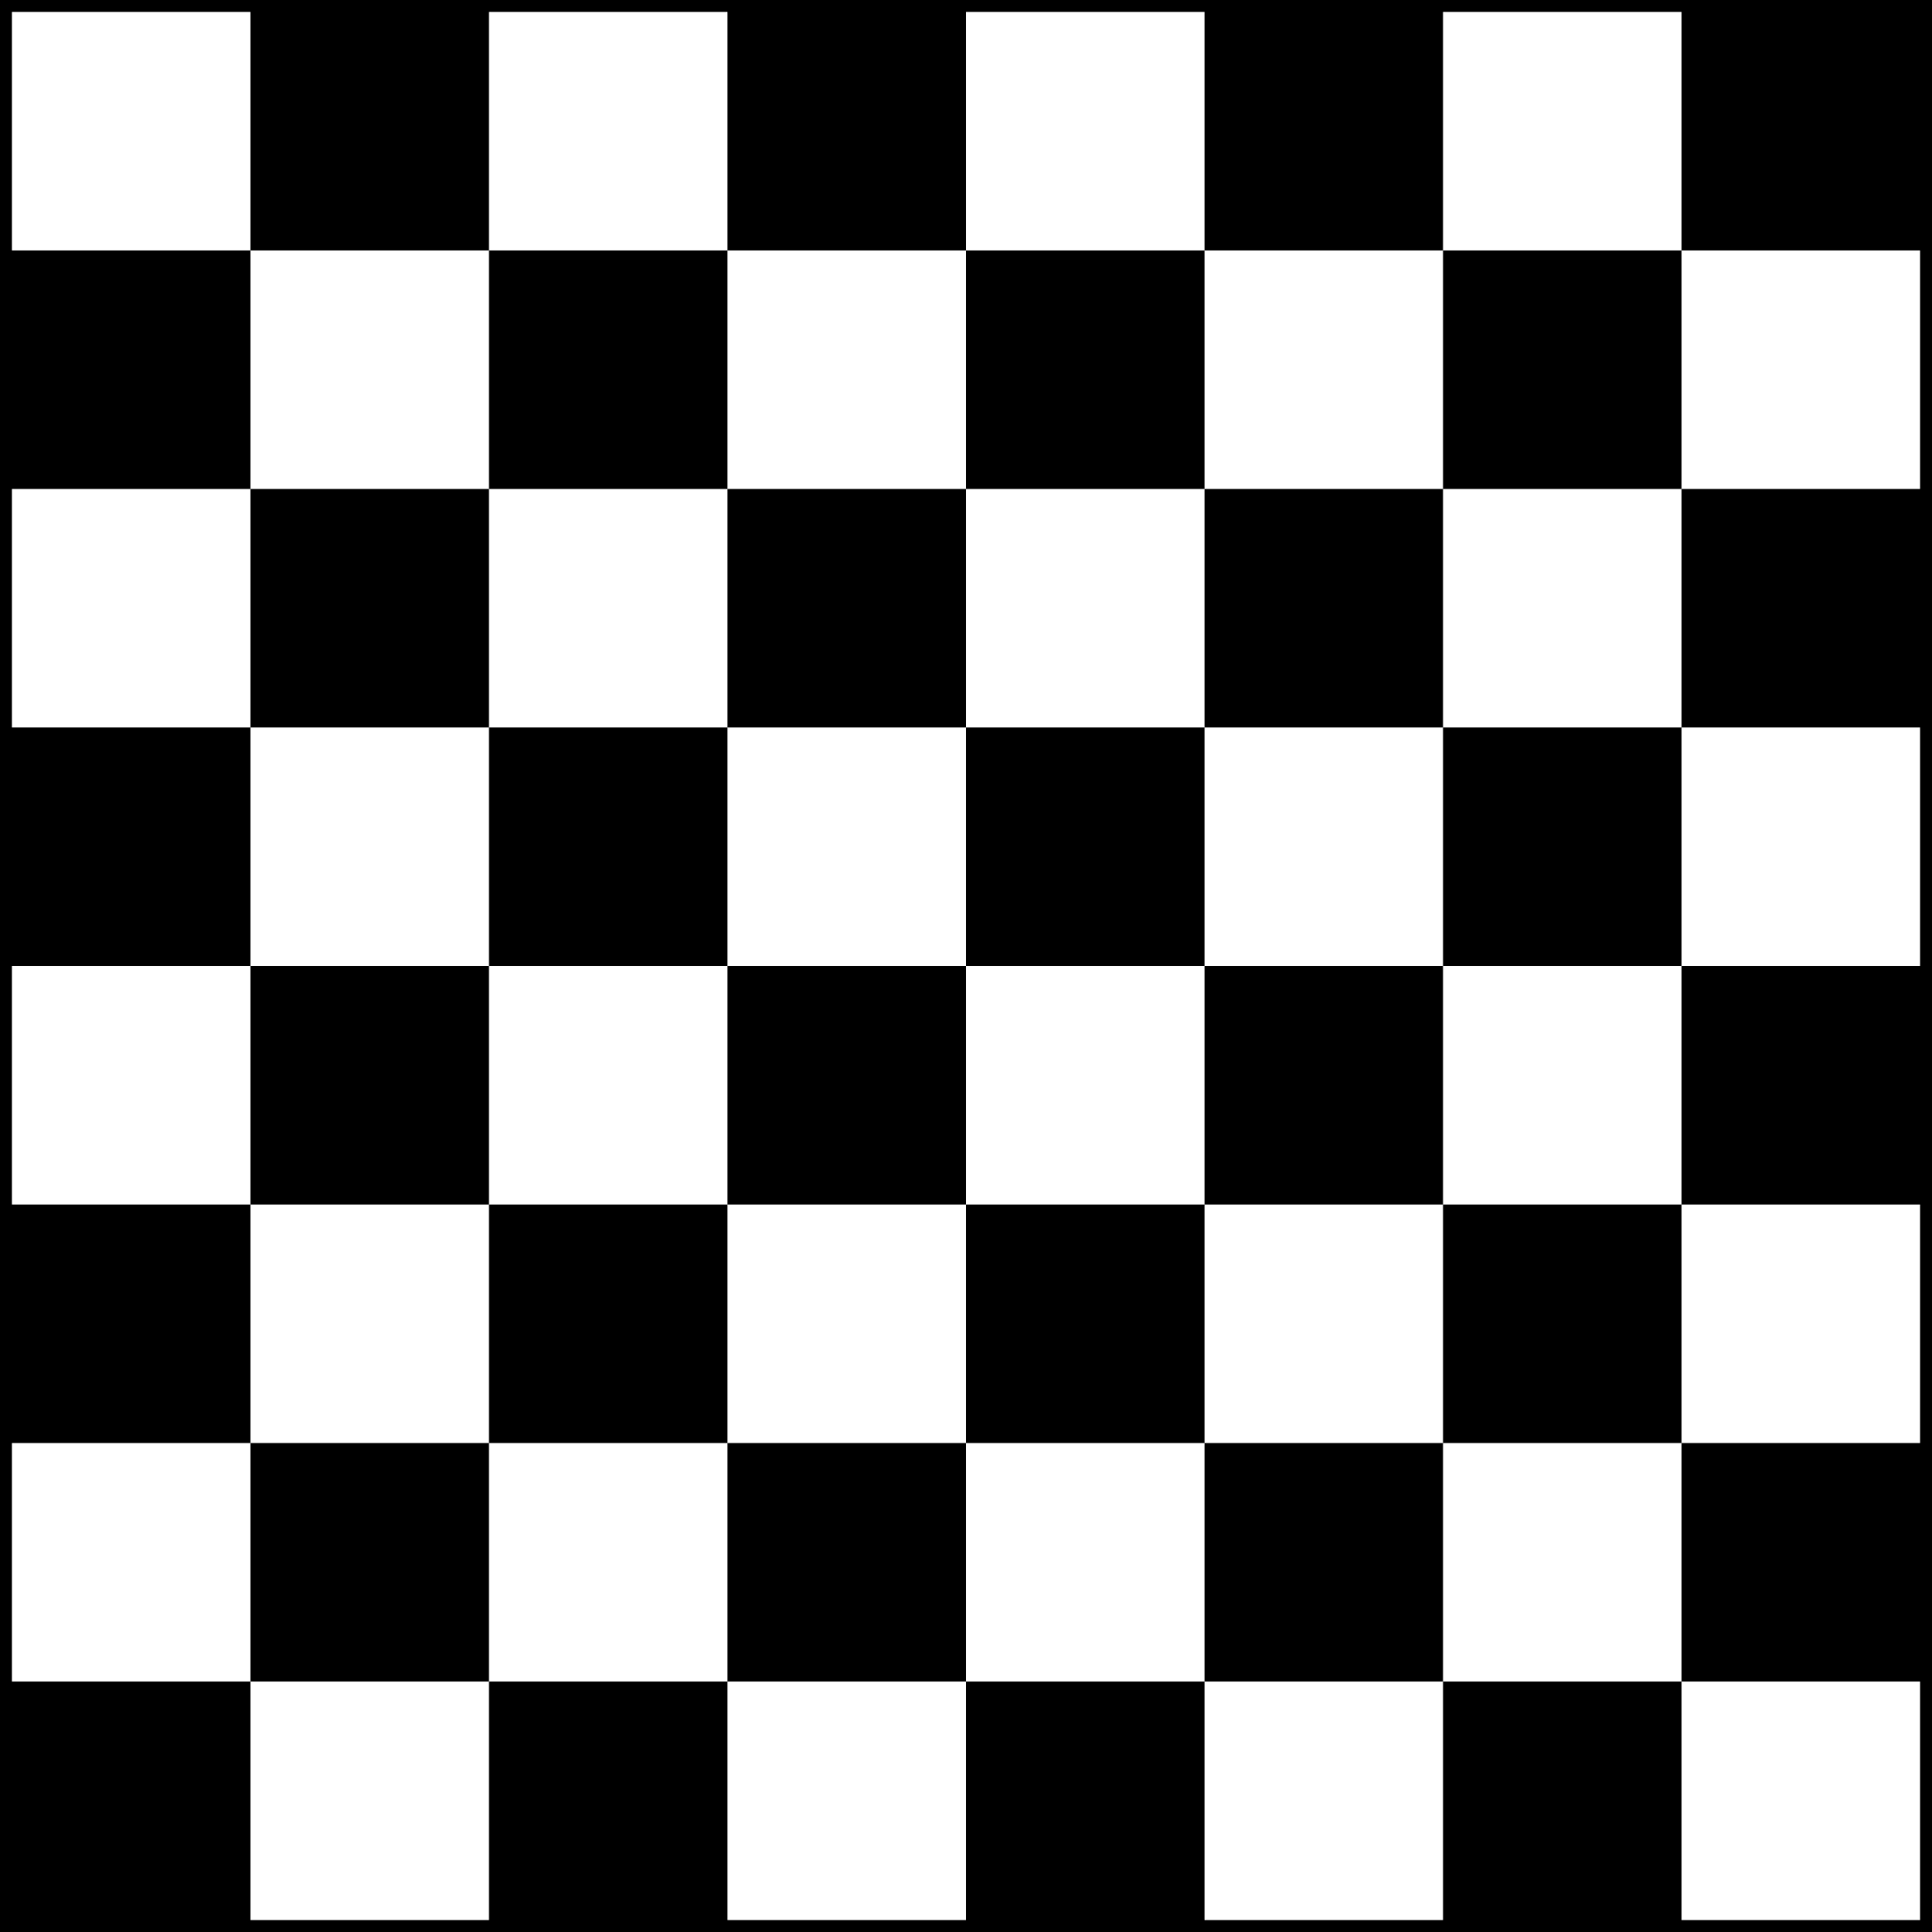
\includegraphics[angle=45,width=4cm]{Chess_Board.png}
\caption{\label{fig:org3cca58f}The Chessboard-Rotated}
\end{figure}

From \ref{fig:org3cca58f}, we can write the array of delta function.

\begin{equation}
\begin{split}
\Delta(x,y) = & \left[\delta(X+1)+\delta(X+3)+\delta(X+5)+\delta(X+7)+\delta(X-1)+\delta(X-3)+\delta(X-5)+\delta(X-7)\right]\delta(Y) \\
& +\left[\delta(X+1)+\delta(X+3)+\delta(X+5)+\delta(X-1)+\delta(X-3)+\delta(X-5)\right][\delta(Y-2)+\delta(Y+2)] \\
& +\left[\delta(X+1)+\delta(X+3)+\delta(X-1)+\delta(X-3)+\right][\delta(Y-2)+\delta(Y+2)+\delta(Y-4)+\delta(Y+4)] \\ 
& +\left[\delta(X+1)+\delta(X-1)+\right][\delta(Y-2)+\delta(Y+2)+\delta(Y-4)+\delta(Y+4)+\delta(Y-6)+\delta(Y+6)] \\ 
\end{split}
\end{equation}

The Fourier Transform of this is,

\begin{equation}
\label{eq:orgc663f33}
\begin{split}
\mathcal{F}\{\Delta(x,y)\} = & 2\left[\cos 2\pi F_X+\cos 6\pi F_X+\cos 10\pi F_X+\cos 14\pi F_X\right] \\
& + 4\left[\cos 2\pi F_X+\cos 6\pi F_X+\cos 10\pi F_X \right]\cos 4\pi F_Y \\
& + 4\left[\cos 2\pi F_X+\cos 6\pi F_X \right]\left[\cos 4\pi F_Y+\cos 8\pi F_Y \right] \\
& + 4\left[\cos 2\pi F_X\right]\left[\cos 4\pi F_Y+\cos 8\pi F_Y +\cos 12\pi F_Y\right]
\end{split}
\end{equation}

We did a coordinate transformation to do this. So we need to do that in the Fourier space also. 

\begin{equation}
\begin{split}
G(f_X,f_Y) = & \iint_{-\infty}^{\infty} dxdy f(x,y) e^{-2i\pi(f_Xx+f_Yy)} \\
= & \frac{1}{4}\iint_{-\infty}^{\infty} dXdY f\left(\left(\frac{X+Y}{2}\right),\left(\frac{X-Y}{2}\right)\right) e^{-2i\pi\left(f_X\left(\frac{X+Y}{2}\right)+f_Y\left(\frac{X-Y}{2}\right)\right)}
\end{split}
\end{equation}

From this, we can say that,

\begin{equation}
\label{eq:org9210cdf}
\begin{split}
F_X = & \frac{f_X+f_Y}{2}\\
F_Y = & \frac{f_X-f_Y}{2}\\
\end{split}
\end{equation}

Apply these to \ref{eq:orgc663f33},

\begin{equation}
\begin{split}
\mathcal{F}\{\Delta(x,y)\} = & 8\left[\cos \pi \left(f_X+f_Y\right)+\cos 3\pi \left(f_X+f_Y\right)+\cos 5\pi \left(f_X+f_Y\right)+\cos 7\pi \left(f_X+f_Y\right)\right] \\
& + 16\left[\cos \pi \left(f_X+f_Y\right)+\cos 3\pi \left(f_X+f_Y\right)+\cos 5\pi \left(f_X+f_Y\right) \right]\cos 2\pi \left(f_X-f_Y\right) \\
& + 16\left[\cos \pi \left(f_X+f_Y\right)+\cos 3\pi \left(f_X+f_Y\right) \right]\left[\cos 2\pi \left(f_X-f_Y\right)+\cos 4\pi \left(f_X-f_Y\right) \right] \\
& + 16\left[\cos \pi \left(f_X+f_Y\right)\right]\left[\cos 2\pi \left(f_X-f_Y\right)+\cos 4\pi \left(f_X-f_Y\right) +\cos 6\pi \left(f_X-f_Y\right)\right]
\end{split}
\end{equation}

For the squre, we can use the result \ref{eq:org485f511}.

The final solution will be product of both.

\begin{equation}
\mathcal{F}\{g(x,y)\} = \mathcal{F}\{\Delta(x,y)\} \times  \text{sinc}(2\pi f_X)\text{sinc}(2\pi f_Y)
\end{equation}

The plot of this is shown in figure \ref{fig:org0e78d47}.
\begin{figure}[t]
\centering
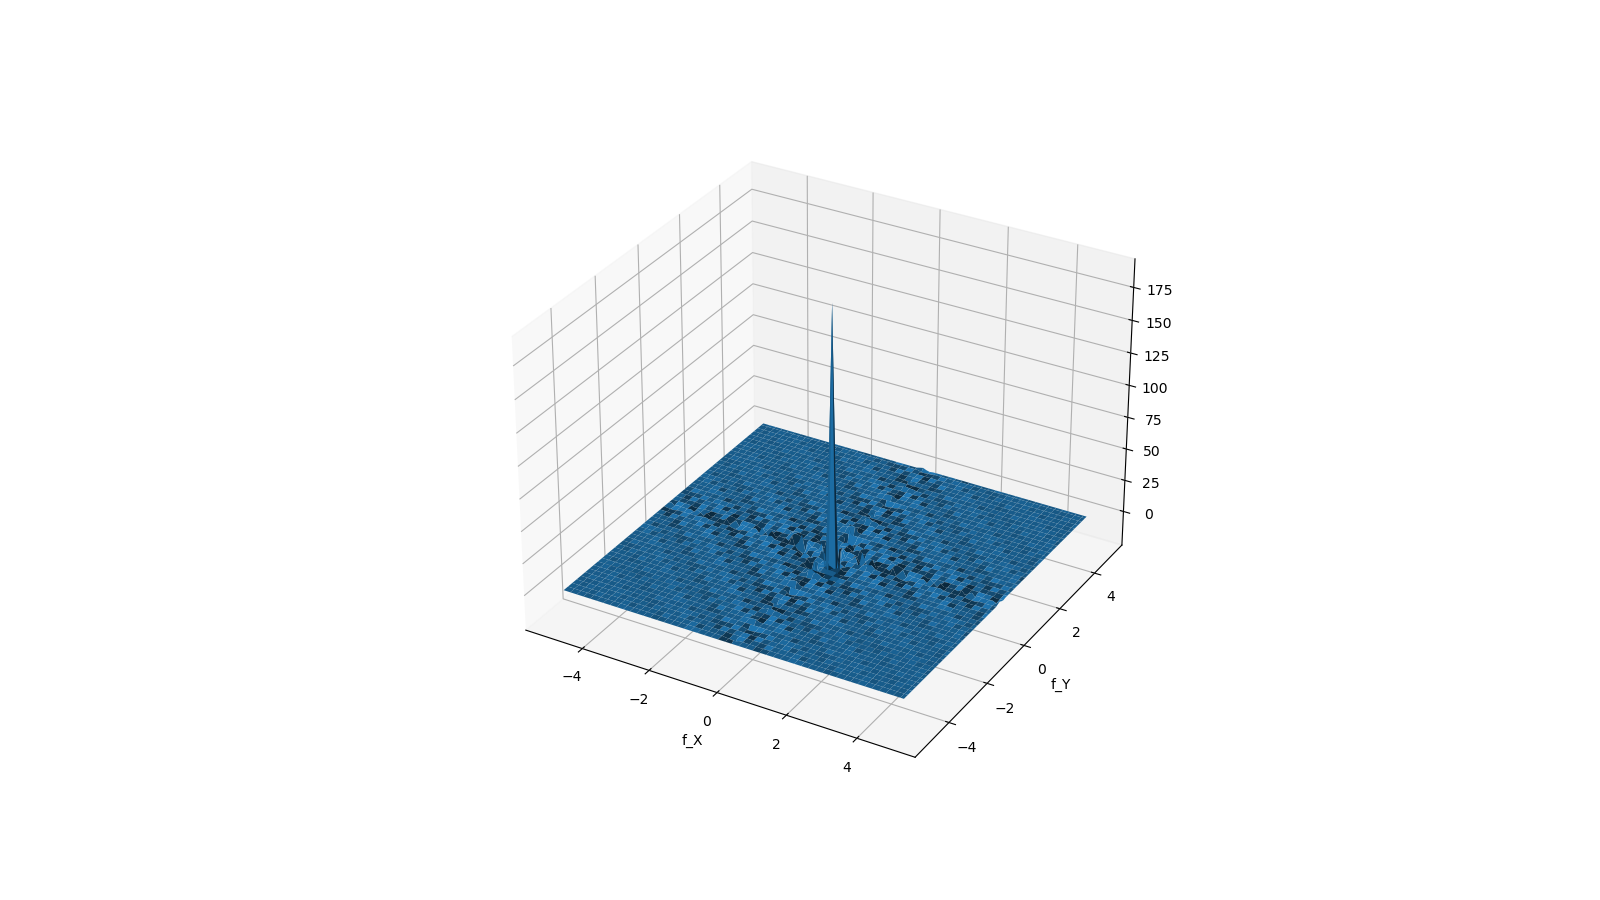
\includegraphics[width=17cm]{3D_plot_pr8.png}
\caption{\label{fig:org0e78d47}3D plot of the Fourier Transform}
\end{figure}
\newpage
\section*{Problem 9}
\label{sec:org84cbfb8}

The visibility \(\nu\) is defined as:
\begin{equation}
\label{eq:orgaeb9f7c}
\nu = \frac{I_{max}-I_{min}}{I_{max}+I_{min}}
\end{equation}
And the degree of coherence can be written as:

\begin{equation}
\label{eq:org921240d}
\gamma(\vec{r_1},\vec{r_2},\tau) = \frac{<f(t)f^*(t+\tau)>}{(I_1I_2)^{\frac{1}{2}}}
\end{equation}

where \(\tau=t_2-t_1\), t\textsubscript{1} and t\textsubscript{2} are the time of arrival of beams from slit to the screen and I\textsubscript{1} = <f(r\textsubscript{1,t})f*(r\textsubscript{1,t})>

For a double slit setup, the total intensity on the screen can be written as

\begin{equation}
\begin{split}
I = & I_1+I_2+(<f_1(t)f_2^*(t+\tau)>)+(<f_1^*(t)f_2(t+\tau)>) \\
= & I_1+I_2+2\mathcal{K}(<f_1(t)f_2^*(t+\tau)>)
\end{split}
\end{equation}

\(\mathcal{K}\) represents a phase factor between f\textsubscript{1} and f\textsubscript{2}. In I\textsubscript{max}, \(\mathcal{K}\) is +1 and I\textsubscript{min}, \(\mathcal{K}\) is -1.

\(\therefore\)

$$I_{max} = I_1+I_2+2(<f_1(t)f_2^*(t+\tau)>)$$
$$I_{min} = I_1+I_2-2(<f_1(t)f_2^*(t+\tau)>)$$

Then, we can write \ref{eq:orgaeb9f7c} as:
\begin{equation}
\label{eq:orgc82c953}
\nu = \frac{2(<f_1(t)f_2^*(t+\tau)>)}{I_1+I_2}
\end{equation}

From \ref{eq:org921240d}, we can now write,

\begin{equation}
\label{eq:org4785aa3}
\nu = \frac{2(I_1I_2)^{\frac{1}{2}}|\gamma(\vec{r_1},\vec{r_2},\tau)|}{I_1+I_2}
\end{equation}

This is the equation that we get which connects degree of coherence and visibility of fringes while the intensity is different. If the intensities are same, \(I_1=I_2\). Then, I\textsubscript{1}+I\textsubscript{2}=2I\textsubscript{1}, I\textsubscript{1I}\textsubscript{2}=I\textsubscript{1}\textsuperscript{2}.

\(\therefore\),

$$\nu = |\gamma(\vec{r_1},\vec{r_2},\tau)|$$

So, our result is consistant with the special case which is given in equestion.

Ref: \url{https://arxiv.org/pdf/1905.00917.pdf}.
$$\star\star\star$$
\end{document}
